\documentclass[11pt,a4paper]{scrarticle}
\usepackage[utf8]{inputenc}
\usepackage{cmap}
\usepackage[T2A]{fontenc}
\usepackage[russian]{babel}
\usepackage{amsmath,amssymb,amsthm,mathtools}
\usepackage{array}

\usepackage{indentfirst}
\usepackage{xcolor,graphicx, tikz, wrapfig}
\usepackage{longtable}
\usepackage{placeins}

\usepackage{minted}
\usemintedstyle{vs}

\usepackage[left=2cm,right=2cm,top=2cm,bottom=2cm,bindingoffset=0cm]{geometry}

\usepackage[unicode]{hyperref}
\definecolor{linkcolor}{HTML}{0000E6}
\definecolor{urlcolor}{HTML}{0000E6}
\definecolor{citecolor}{HTML}{0000E6}
% \hypersetup{pdfpagemode=None,linktoc=page,citecolor=citecolor,linkcolor=linkcolor,urlcolor=urlcolor,colorlinks=true}

\theoremstyle{definition}
\newtheorem{subtask}{Пункт}

\DeclareMathOperator*{\argmax}{arg\,max}
\DeclareMathOperator*{\argmin}{arg\,min}
\newcommand{\floor}[1]{\left\lfloor #1 \right\rfloor}
\newcommand{\ceil}[1]{\left\lceil #1 \right\rceil}


\setlength{\parindent}{1cm}

\author{Клычков Максим Дмитриевич}

\begin{document}

\centerline{\textbf{\huge Алгоритмы и структуры данных-2}}
\centerline{\textbf{SET 6. Задача A1.}}
\begin{flushright}
    \emph{Весна 2024. Клычков М. Д.}
\end{flushright}

\begin{figure}[htp]
    \centering
    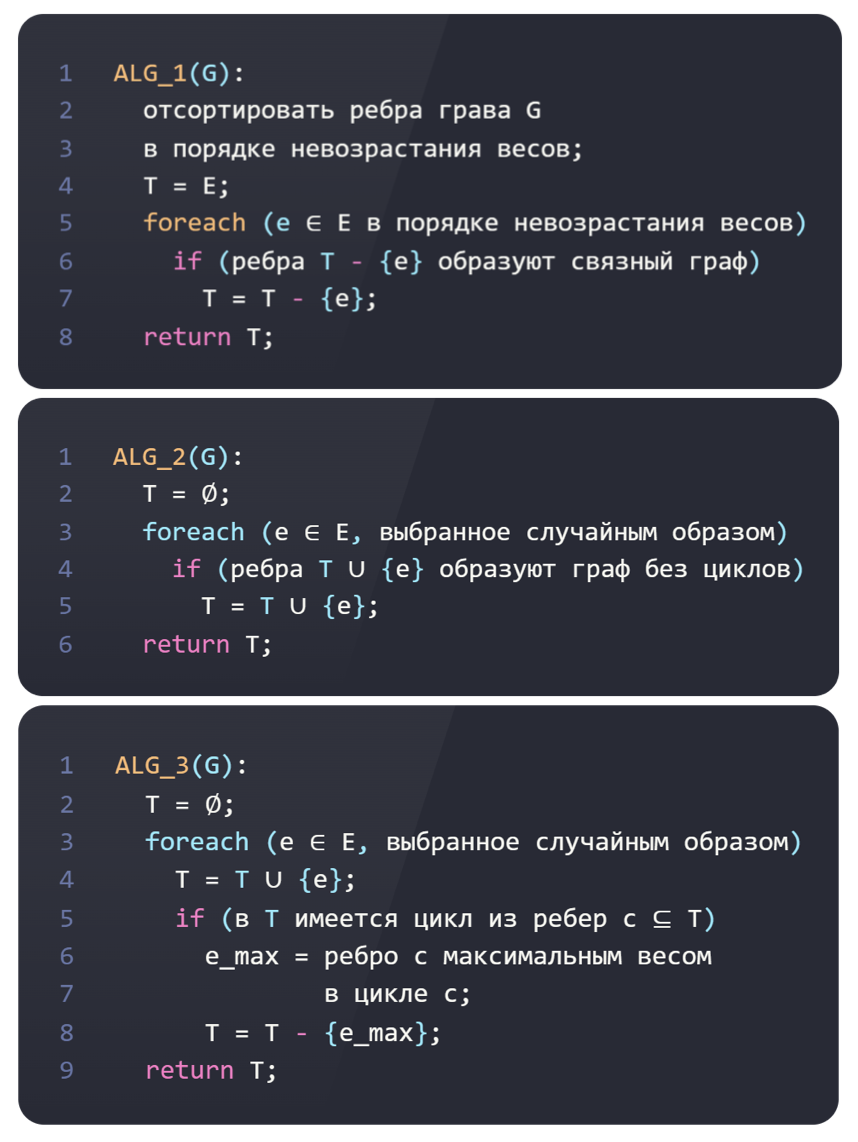
\includegraphics[width=0.4\textwidth]{static/code.png}
    \caption{Код из условия}
    \label{fig:code}
\end{figure}

\begin{subtask}
    Сделаем некоторые предварительные шаги — интерфейс, которым будем пользоваться в некоторых реализациях:

    \begin{minted}
    [
    frame=lines,
    framesep=2mm,
    baselinestretch=1.2,
    fontsize=\footnotesize,
    linenos
    ]
    {cpp}
struct Edge {
  int u;
  int v;
  int weight;
};

class DSU {
 public:
  explicit DSU(int n);
  int Union(int x, int y);
  int Find(int x);
};

using Edges = std::vector<Edge>;
using AdjListItem = std::pair<int, int>;  // pair (to, weight)
using AdjLists = std::vector<std::list<AdjListItem>>;

Edges edges;   // массив ребер
AdjLists adj;  // списки смежности

void Dfs(int u, const AdjLists& adj, std::vector<bool>& visited) {
  visited[u] = true;
  for (auto [v, weight] : adj[u]) {
    if (!visited[v]) {
      Dfs(v, adj, visited);
    }
  }
}

bool IsConnected(const AdjLists& adj_matrix) {
  std::vector<bool> visited(adj_matrix.size());

  Dfs(0, adj_matrix, visited);

  for (bool v : visited) {
    if (!v) {
      return false;
    }
  }
  return true;
}
    \end{minted}

    Последовательно рассмотрим каждую из предложенных функций:
    \begin{itemize}
        \item \texttt{ALG\_1:} для реализации этого алгоритма представим граф в виде списка смежности и массива ребер. Проверять граф на связность будем, используя обход в глубину.

              \begin{minted}
        [
        frame=lines,
        framesep=2mm,
        baselinestretch=1.2,
        fontsize=\footnotesize,
        linenos
        ]
        {cpp}
std::pair<AdjLists, int> ALG_1(Edges& edges, AdjLists adj) {
  AdjLists mst = std::move(adj);  // adj copied in function call
  std::sort(edges.begin(), edges.end(), [](auto e1, auto e2) { return e1.weight > e2.weight; });
  int cost = 0;

  for (auto [u, v, weight] : edges) {
    // remove edge uv from mst
    mst[u].remove({v, weight});
    mst[v].remove({u, weight});

    if (!IsConnected(mst)) {
      // add edge uv back to mst
      mst[u].emplace_back(v, weight);
      mst[v].emplace_back(u, weight);
      cost += weight;
    }
  }

  return {mst, cost};
}
        \end{minted}

              Временная сложность такого алгоритма будет $O(E \log E + (E \cdot (V + E)))$. Действительно, оптимальная сортировка занимает $O(E \log E)$, а сам алгоритм перебирает все ребра и на каждом шаге проверяет связность графа с помощью обхода в глубину, который занимает $O(V + E)$. Можно еще упомянуть тот факт, что удаление из листа занимает линейное относительно количества вершин время, однако это уже учтено в объявленной временной сложности (просто выражается в константе).

              Достаточно очевидно, что такой главная проблема такого подхода — проверка на связность. Можно найти подтверждение того, что проверка связности при последовательном удалении ребер решается задачей \textbf{Fully-dynamic graph problem}, решение которой позволяет быстро проверять граф на связность при вставках и удалениях ребер (\textit{как раз то, что нам нужно!}). Мною было найдено решение этой задачи за $O(\log V (\log \log V)^3)$. Тогда общая сложность будет $O(E \log E + (\log V (\log \log V)^3))$.

        \item \texttt{ALG\_2:} для реализации этого алгоритма представим граф массива ребер. Для проверки графа на ацикличность будем использовать структуру \textbf{Система непересекающихся множеств}.

              \begin{minted}
        [
        frame=lines,
        framesep=2mm,
        baselinestretch=1.2,
        fontsize=\footnotesize,
        linenos
        ]
        {cpp}
std::pair<Edges, int> ALG_2(Edges& edges, int n) {
  std::shuffle(edges.begin(), edges.end(), std::default_random_engine{});
  Edges mst{};
  DSU dsu{n};
  int cost = 0;

  for (auto e : edges) {
    if (dsu.Find(e.u) != dsu.Find(e.v)) {
      mst.push_back(e);
      dsu.Union(e.u, e.v);
      cost += e.weight;
    }
  }

  return {mst, cost};
}
        \end{minted}

              Предварительно совершается шаффл массива ребер — не будем учитывать его при анализе общей сложности, но уточним, что такая операция занимает $O(n)$ свапов в массиве.

              Сам алгоритм представляет из себя перебор всех ребер в графе, где на каждом шаге выполняется одна-две операции на структуре Система непересекающихся множеств. Известно, что оптимальная реализация такой структуры позволяет совершать операции \texttt{UNION} и \texttt{FIND} за $O(\alpha(V))$, где $\alpha(n)$ — обратная функция Аккермана. Тогда итоговая временная сложность алгоритма $O(E \cdot \alpha(V))$

        \item \texttt{ALG\_3:} В реализации этого алгоритма — придумать, как реализовать поиск самого тяжелого ребра в образовавшемся цикле. Имеющихся знаний хватает только на идею прохода по всему циклу с помощью обхода в глубину. Циклы все также с использованием DSU. Для хранения графа будем использовать список смежности и массив ребер.

              Реализация поиска цикла в графе может быть следующей:
              \begin{minted}
        [
        frame=lines,
        framesep=2mm,
        baselinestretch=1.2,
        fontsize=\footnotesize,
        linenos
        ]
        {cpp}
std::vector<int> FindCycle(int from) {
  std::vector<int> cycle;
  std::vector<bool> visited(adj.size());
  std::vector<int> parent(adj.size(), -1);

  std::function<bool(int)> dfs = [&](int u) {
    visited[u] = true;
    for (auto [v, weight] : adj[u]) {
      if (!visited[v]) {
        parent[v] = u;
        if (dfs(v)) {
          return true;
        }
      } else if (v != parent[u]) {
        cycle.push_back(u);
        for (int i = u; i != v; i = parent[i]) {
          cycle.push_back(i);
        }
        cycle.push_back(v);
        return true;
      }
    }
    return false;
  };

  dfs(from);
  return cycle;
}
        \end{minted}

              Тогда сам алгоритм будет выглядеть следующим образом:
              \begin{minted}
        [
        frame=lines,
        framesep=2mm,
        baselinestretch=1.2,
        fontsize=\footnotesize,
        linenos
        ]
        {cpp}
std::pair<AdjLists, int> ALG_3(Edges& edges, int n) {
  AdjLists mst(n);
  std::shuffle(edges.begin(), edges.end(), std::default_random_engine{});
  DSU dsu{n};
  int cost = 0;

  for (auto e : edges) {
    if (dsu.Find(e.u) != dsu.Find(e.v)) {
      mst[e.u].emplace_back(e.v, e.weight);
      mst[e.v].emplace_back(e.u, e.weight);
    } else {
      auto cycle = FindCycle(e.u);
      int max_weight = 0;
      int to_remove_start = -1, to_remove_end = -1;
      for (int i = 0; i < cycle.size() - 1; ++i) {
        int u = cycle[i];
        int v = cycle[i + 1];
        int new_weight = std::find_if(edges.begin(), edges.end(), [&](auto e) {
                           return (e.u == u && e.v == v) || (e.u == v && e.v == u);
                         })->weight;
        if (new_weight > max_weight) {
          max_weight = new_weight;
          to_remove_start = u;
          to_remove_end = v;
        }
      }

      if (max_weight > e.weight) {
        mst[to_remove_start].remove({to_remove_end, max_weight});
        mst[to_remove_end].remove({to_remove_start, max_weight});
        mst[e.u].emplace_back(e.v, e.weight);
        mst[e.v].emplace_back(e.u, e.weight);
        cost += e.weight - max_weight;
      }
    }
  }

  return {mst, cost};
}
        \end{minted}

              Получается, что мы идем по всем ребрам $O(E)$ и на каждой итерации либо добавляем ребро в дерево, либо ищем цикл и удаляем самое тяжелое ребро в нем. Поиск цикла занимает $O(V + E)$, а поиск самого тяжелого ребра в цикле — $O(E)$. Также на каждой итерации пользуемся «оптимальным» \texttt{DSU} за обратную функцию Аккермана. Тогда итоговая временная сложность алгоритма $O(E \cdot (\alpha(V) + V + E))$. Заметим, что вполне можно было бы обойтись без структуры \texttt{DSU} (\textit{даже асимптотика была бы лучше!}), однако ее использование позволяет не запускать медленный \texttt{DFS} для поиска цикла на каждом шаге.
    \end{itemize}
\end{subtask}

\begin{subtask}
    Теперь проверим корректность каждого из алгоритмов.

    \begin{itemize}
        \item \texttt{ALG\_1:} Легко показать, что полученный с помощью удалений подграф $T$ является деревом. Действительно, если на каком-то шаге алгоритма есть цикл, то на одном из последующих шагов мы найдем самое тяжелое ребро в этом цикле и удалим его, так как это не нарушит связности. Формально минимальность можно доказать по индукции, однако, по-мнению автора, достаточно и интуиции. Уже доказано (точнее является следствием), что все оставшиеся ребра являются \textit{light}-ребрами. Пусть есть какое-то более дешевое \textit{light}-ребро $e$, не входящее в $T$, но так как исходно ребра были отсортированы по убыванию, все тяжелые ребра были удалены, получается, что $e \in T$.

        \item \texttt{ALG\_2:} Этот алгоритм в точности повторяет алгоритм Краскала, за исключением упорядоченности массива, что и является ключевой идеей в построении \textbf{Минимального} остовного дерева. В качестве контрпримера достаточно взять простой цикл на трех вершинах (\textit{треугольник}) с различными взвешенными ребрами. Очевидно, что ответ \texttt{ALG\_2} не всегда будет корректным.

        \item \texttt{ALG\_3:} Очевидно, что полученный в алгоритме граф является деревом (связным графом без циклов), так как все циклы в нем мы разрушили удалением ребер при обнаружении (одно ребро может образовать лишь один цикл). Далее минимальность — алгоритм работает по принципу жадного выбора: на каждом шаге он делает локально оптимальное решение (удаляет максимальное ребро в цикле), что в итоге приводит к глобально оптимальному решению (минимальному остовному дереву). Если бы существовало другое остовное дерево с меньшим весом, это означало бы, что на каком-то шаге алгоритм оставил ребро с большим весом, чем необходимо. Однако это невозможно, так как алгоритм всегда удаляет максимальное ребро в цикле.
    \end{itemize}
\end{subtask}

\end{document}

